Pe langa facilitatile de extensibilitate oferite de utilizarea serviciilor cloud din cadrul "Amazon Web Services", arhitectura aplicatiei "Surf" prezinta urmatoarele puncte de extensie:

\begin{itemize}
	\item{Adaugare rapida si usoara de noi servicii cloud in cluster-ul aplicatiei, datorita structurii decuplate si configurabile a mecanismului de generare a infrastructurii;}
	\item{Asigurarea infrastructurii crawler-ului in mai multe regiuni globale, in conformitate cu politicile de globalizare AWS, astfel incat aplicatia "Surf" sa poata fi folosita la scara larga;}
	\item{Posibilitatea de a adauga functii Lambda de tip plug-in in cadrul mecanismului de parcurgere si procesare a informatiilor din cadrul paginilor web vizitate de catre crawler (\textit{"Figura 11"}).}
\end{itemize}

\begin{figure}[ht]
\begin{center}
	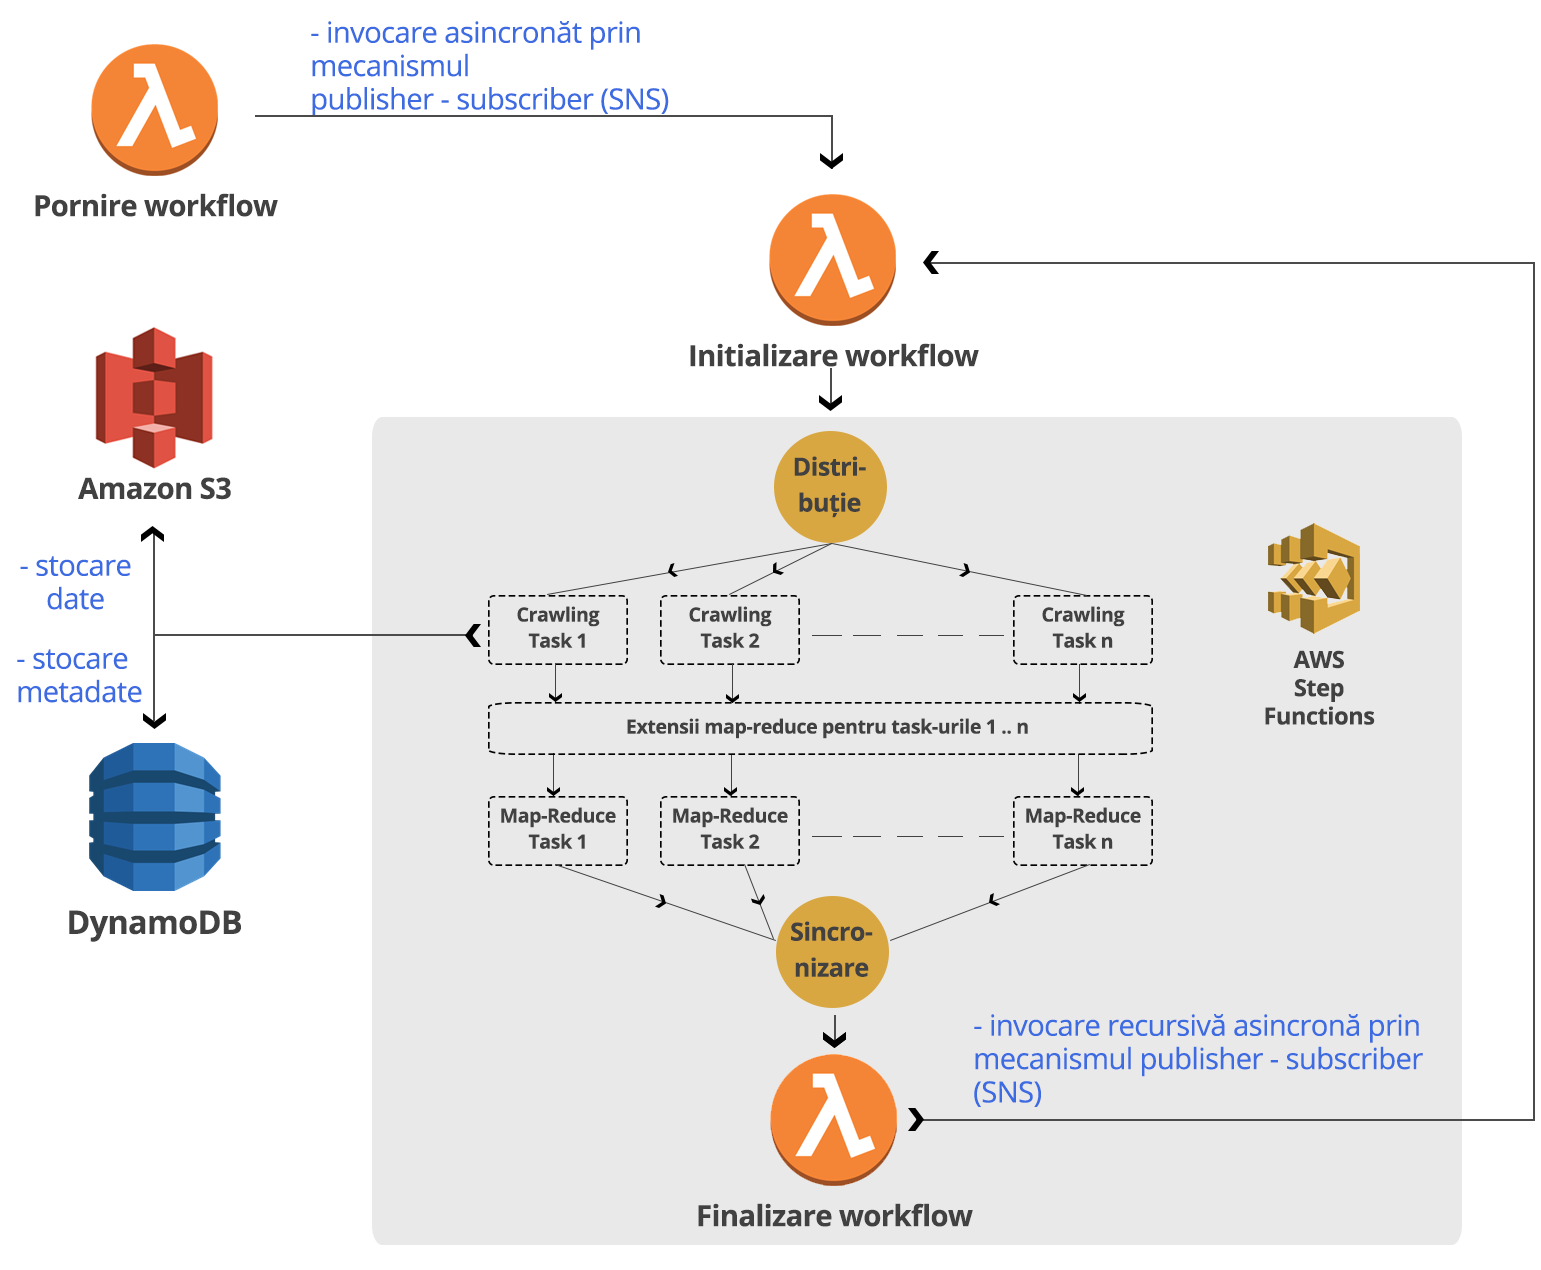
\includegraphics[keepaspectratio, width=0.9\textwidth]{proces-crawling-cu-pluginuri.png}
	\caption{Plugin-uri adaugate procesului de crawling \cite{diagram-icons-sources, aws-icons-source}}\par\medskip 

\end{center}
\end{figure}